

\chapter{Miro Usage}
\label{apendixMiroUsage}

As a reference, three screenshots of the Miro board at different stages of this project are provided. They show the increase in information as well as the restructuring of information blocks. Three observations can be made. First, the zoom level required to display the entire board on one screen had to be increased multiple times due to the growing number of meetings, Kanban cards, and other elements. Second, the implementation and document writing section in the bottom right grew considerably compared to the first screenshot. Third, new information was added continuously, which can be seen mainly in the bottom right. Finally, after these reference screenshots, some sections are highlighted to show readable parts of the work carried out on the board.


\begin{figure}[H]
    \centering
    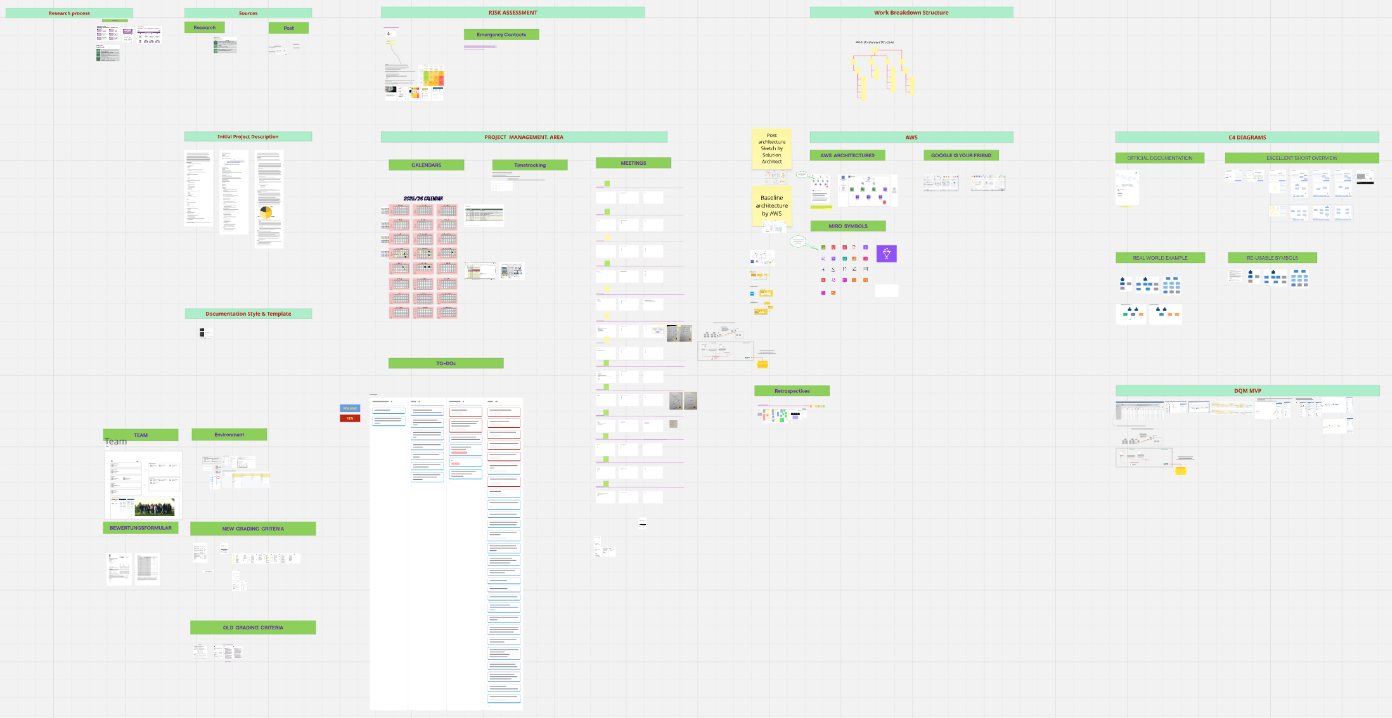
\includegraphics[width=0.8\textwidth]{./content/img/MiroBoard__Old_10-11-2025.png}
    \caption{Miro board documentation, view of 10.11.2025}
    \label{fig:miro_board_tenth_november}
\end{figure}

\begin{figure}[H]
    \centering
    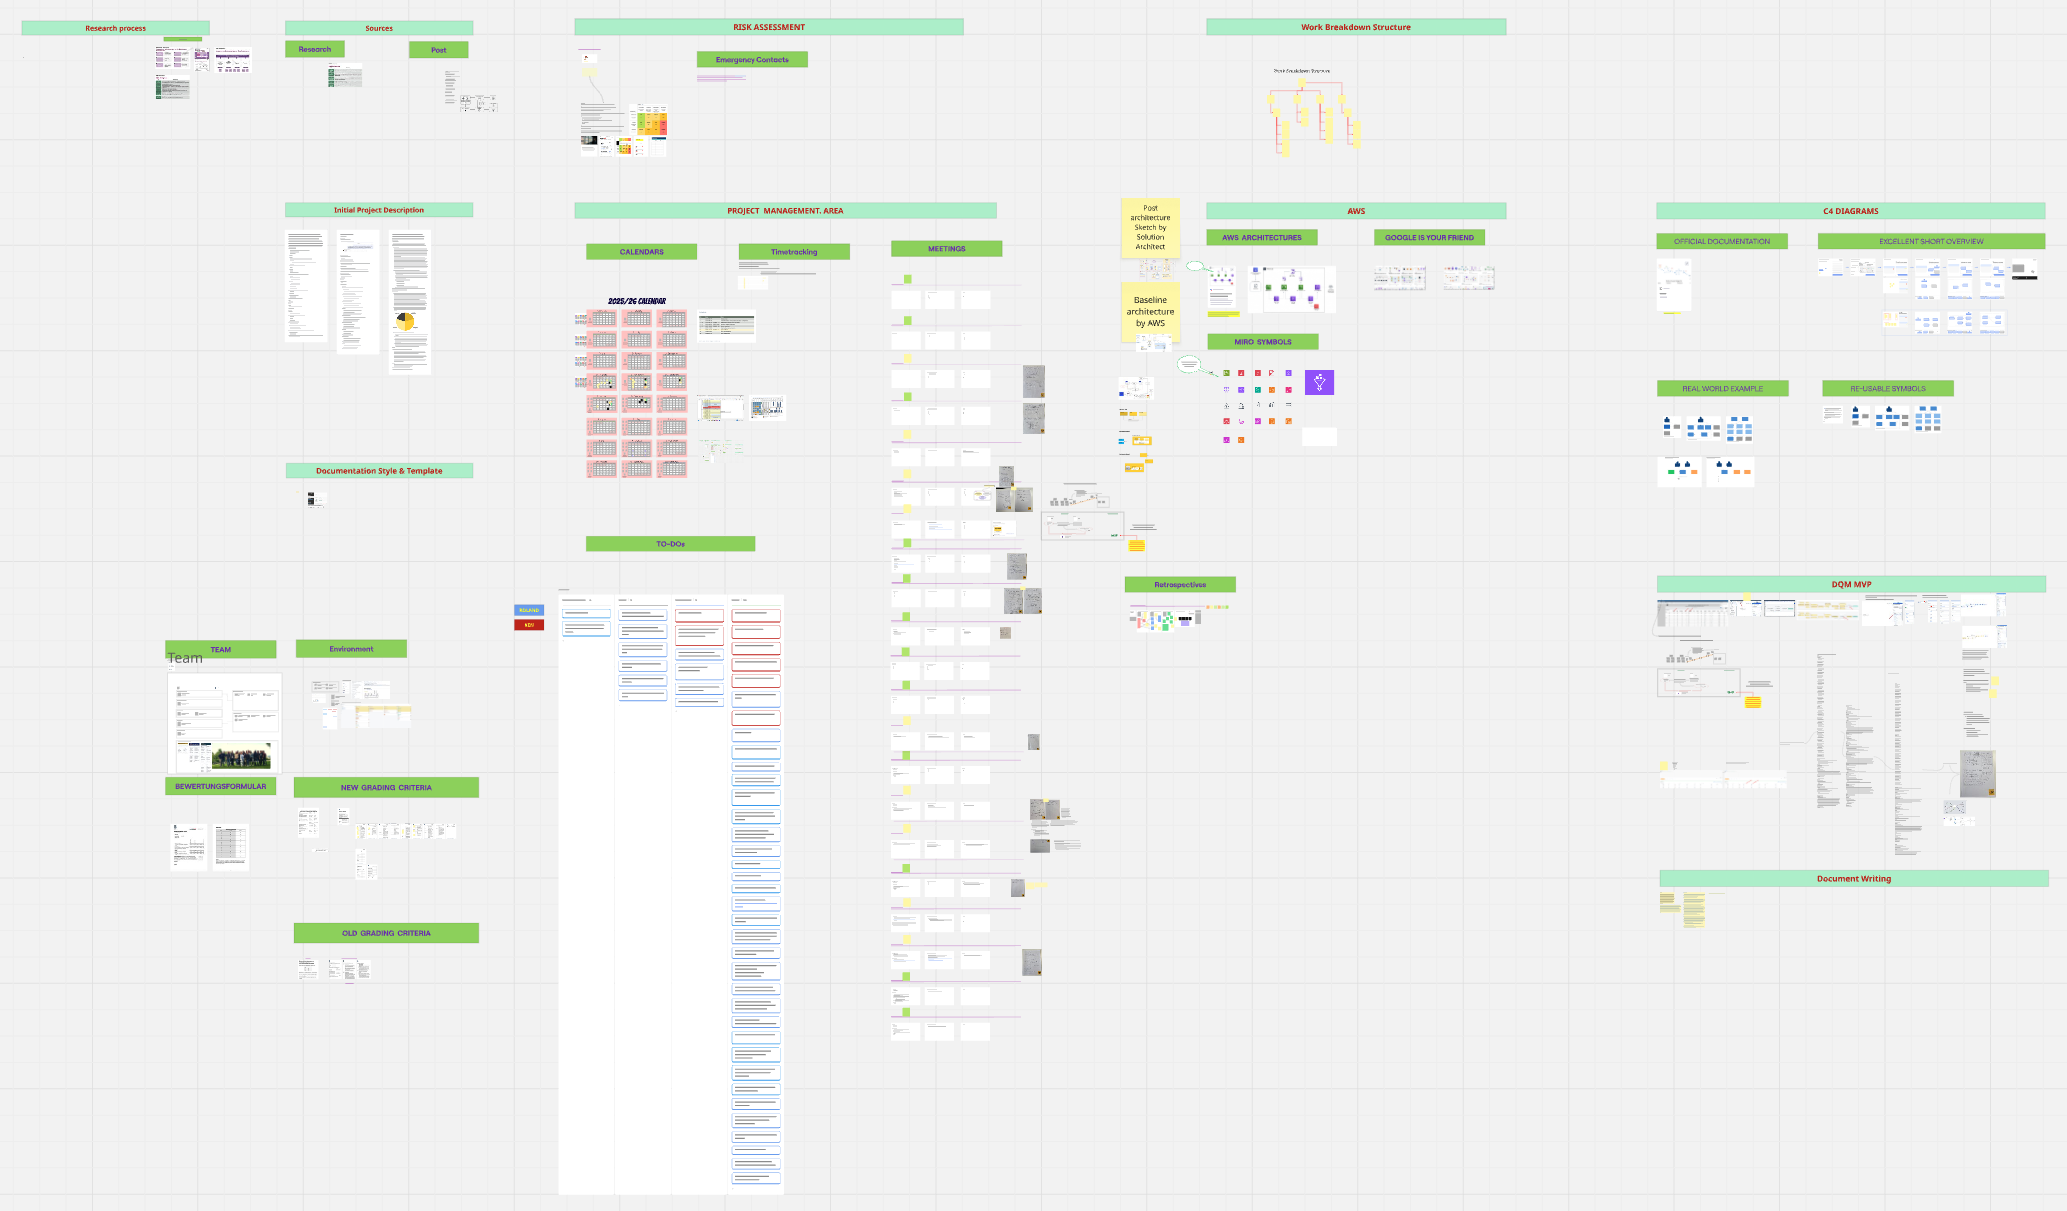
\includegraphics[width=0.8\textwidth]{./content/img/MiroBoard_25-11-2025_15-36-28.png}
    \caption{Miro board documentation, view of 25.11.2025}
    \label{fig:miro_board_twentyfifth_november}
\end{figure}

\begin{figure}[H]
    \centering
    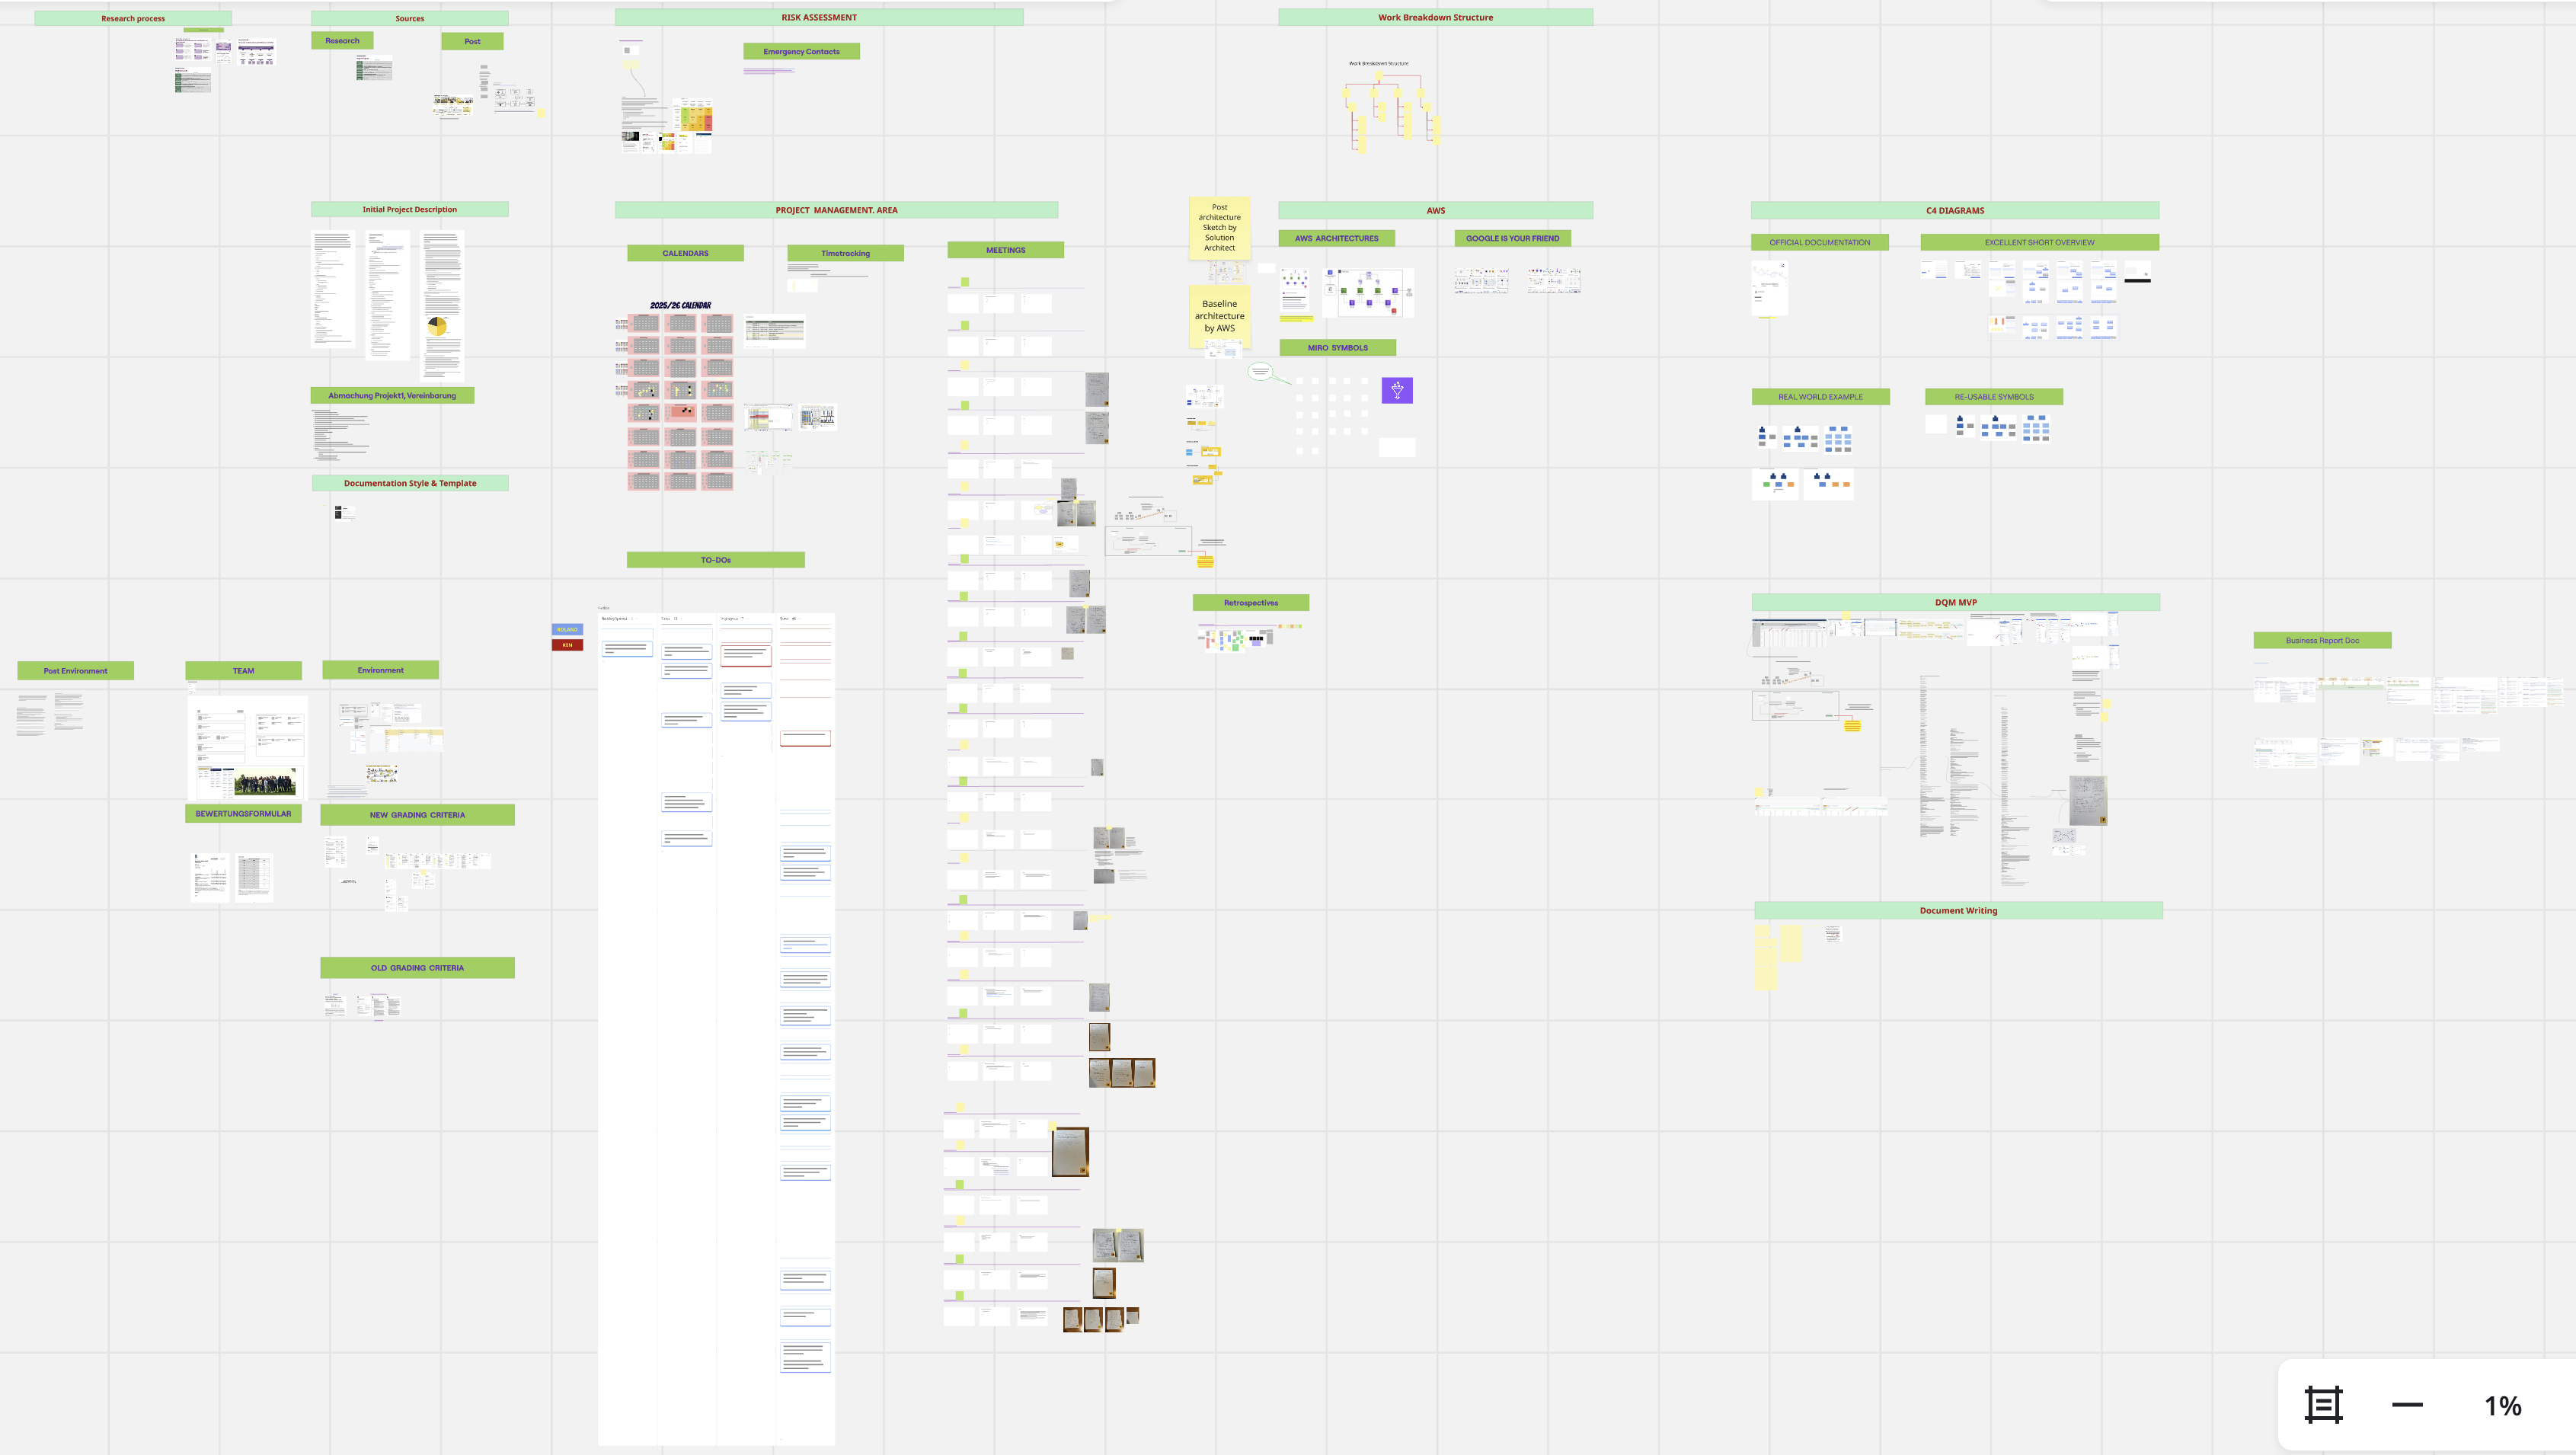
\includegraphics[width=0.8\textwidth]{./content/img/MiroBoard_23-12-2025.png}
    \caption{Miro board documentation, view of 23.12.2025}
    \label{fig:miro_board_twentythird_december}
\end{figure}

\begin{figure}[H]
    \centering
    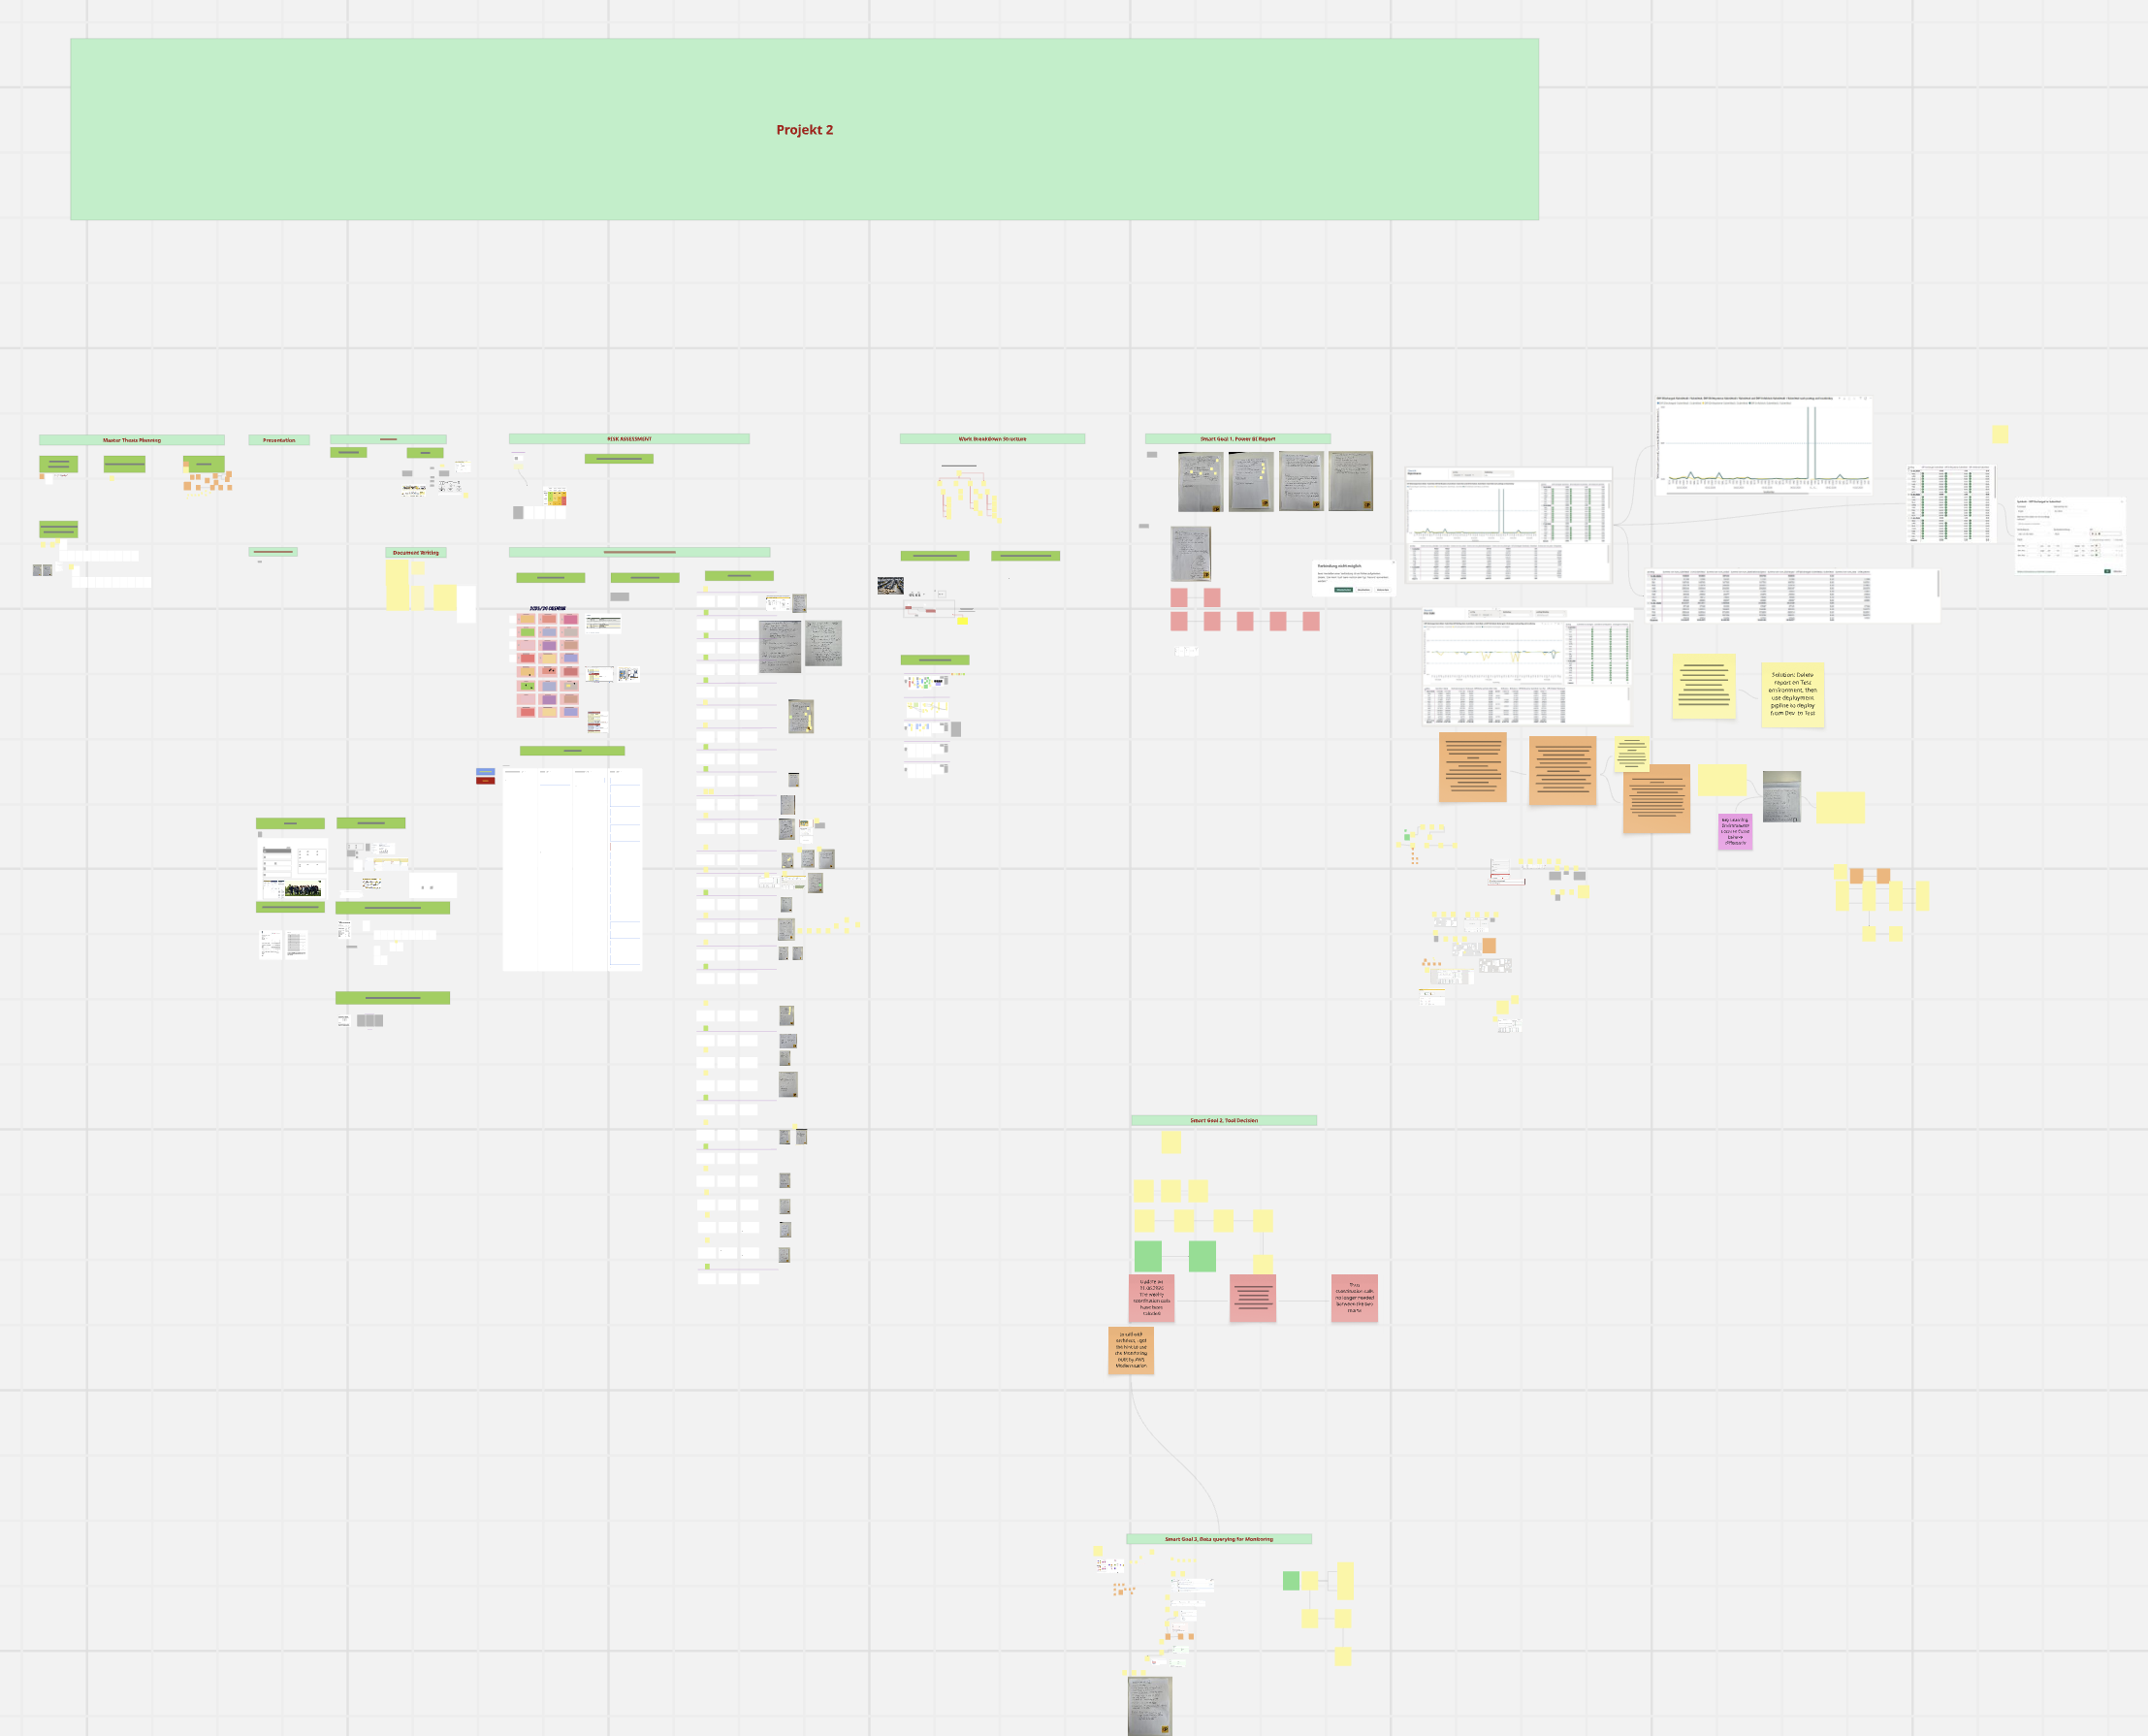
\includegraphics[width=\textwidth]{./content/img/MiroBoard_24_07_2026png.png}
    \caption{Complete Miro board documenting the evolution of the project. The board contains the complete collection of notes, diagrams, screenshots, milestones, implementation artefacts and planning information accumulated during the project. Screenshot taken on 24 July 2026.}
    \label{fig:annex_miro_complete}
\end{figure}


\section{Miro Details of SMART Goals}

The following screenshots provide a high-level overview of the work carried out for the individual SMART Goals. These screenshots are intended only as a reference and are not meant to be readable in detail, but rather to provide a brief overview of the methods used.



\begin{figure}[H]
    \centering
    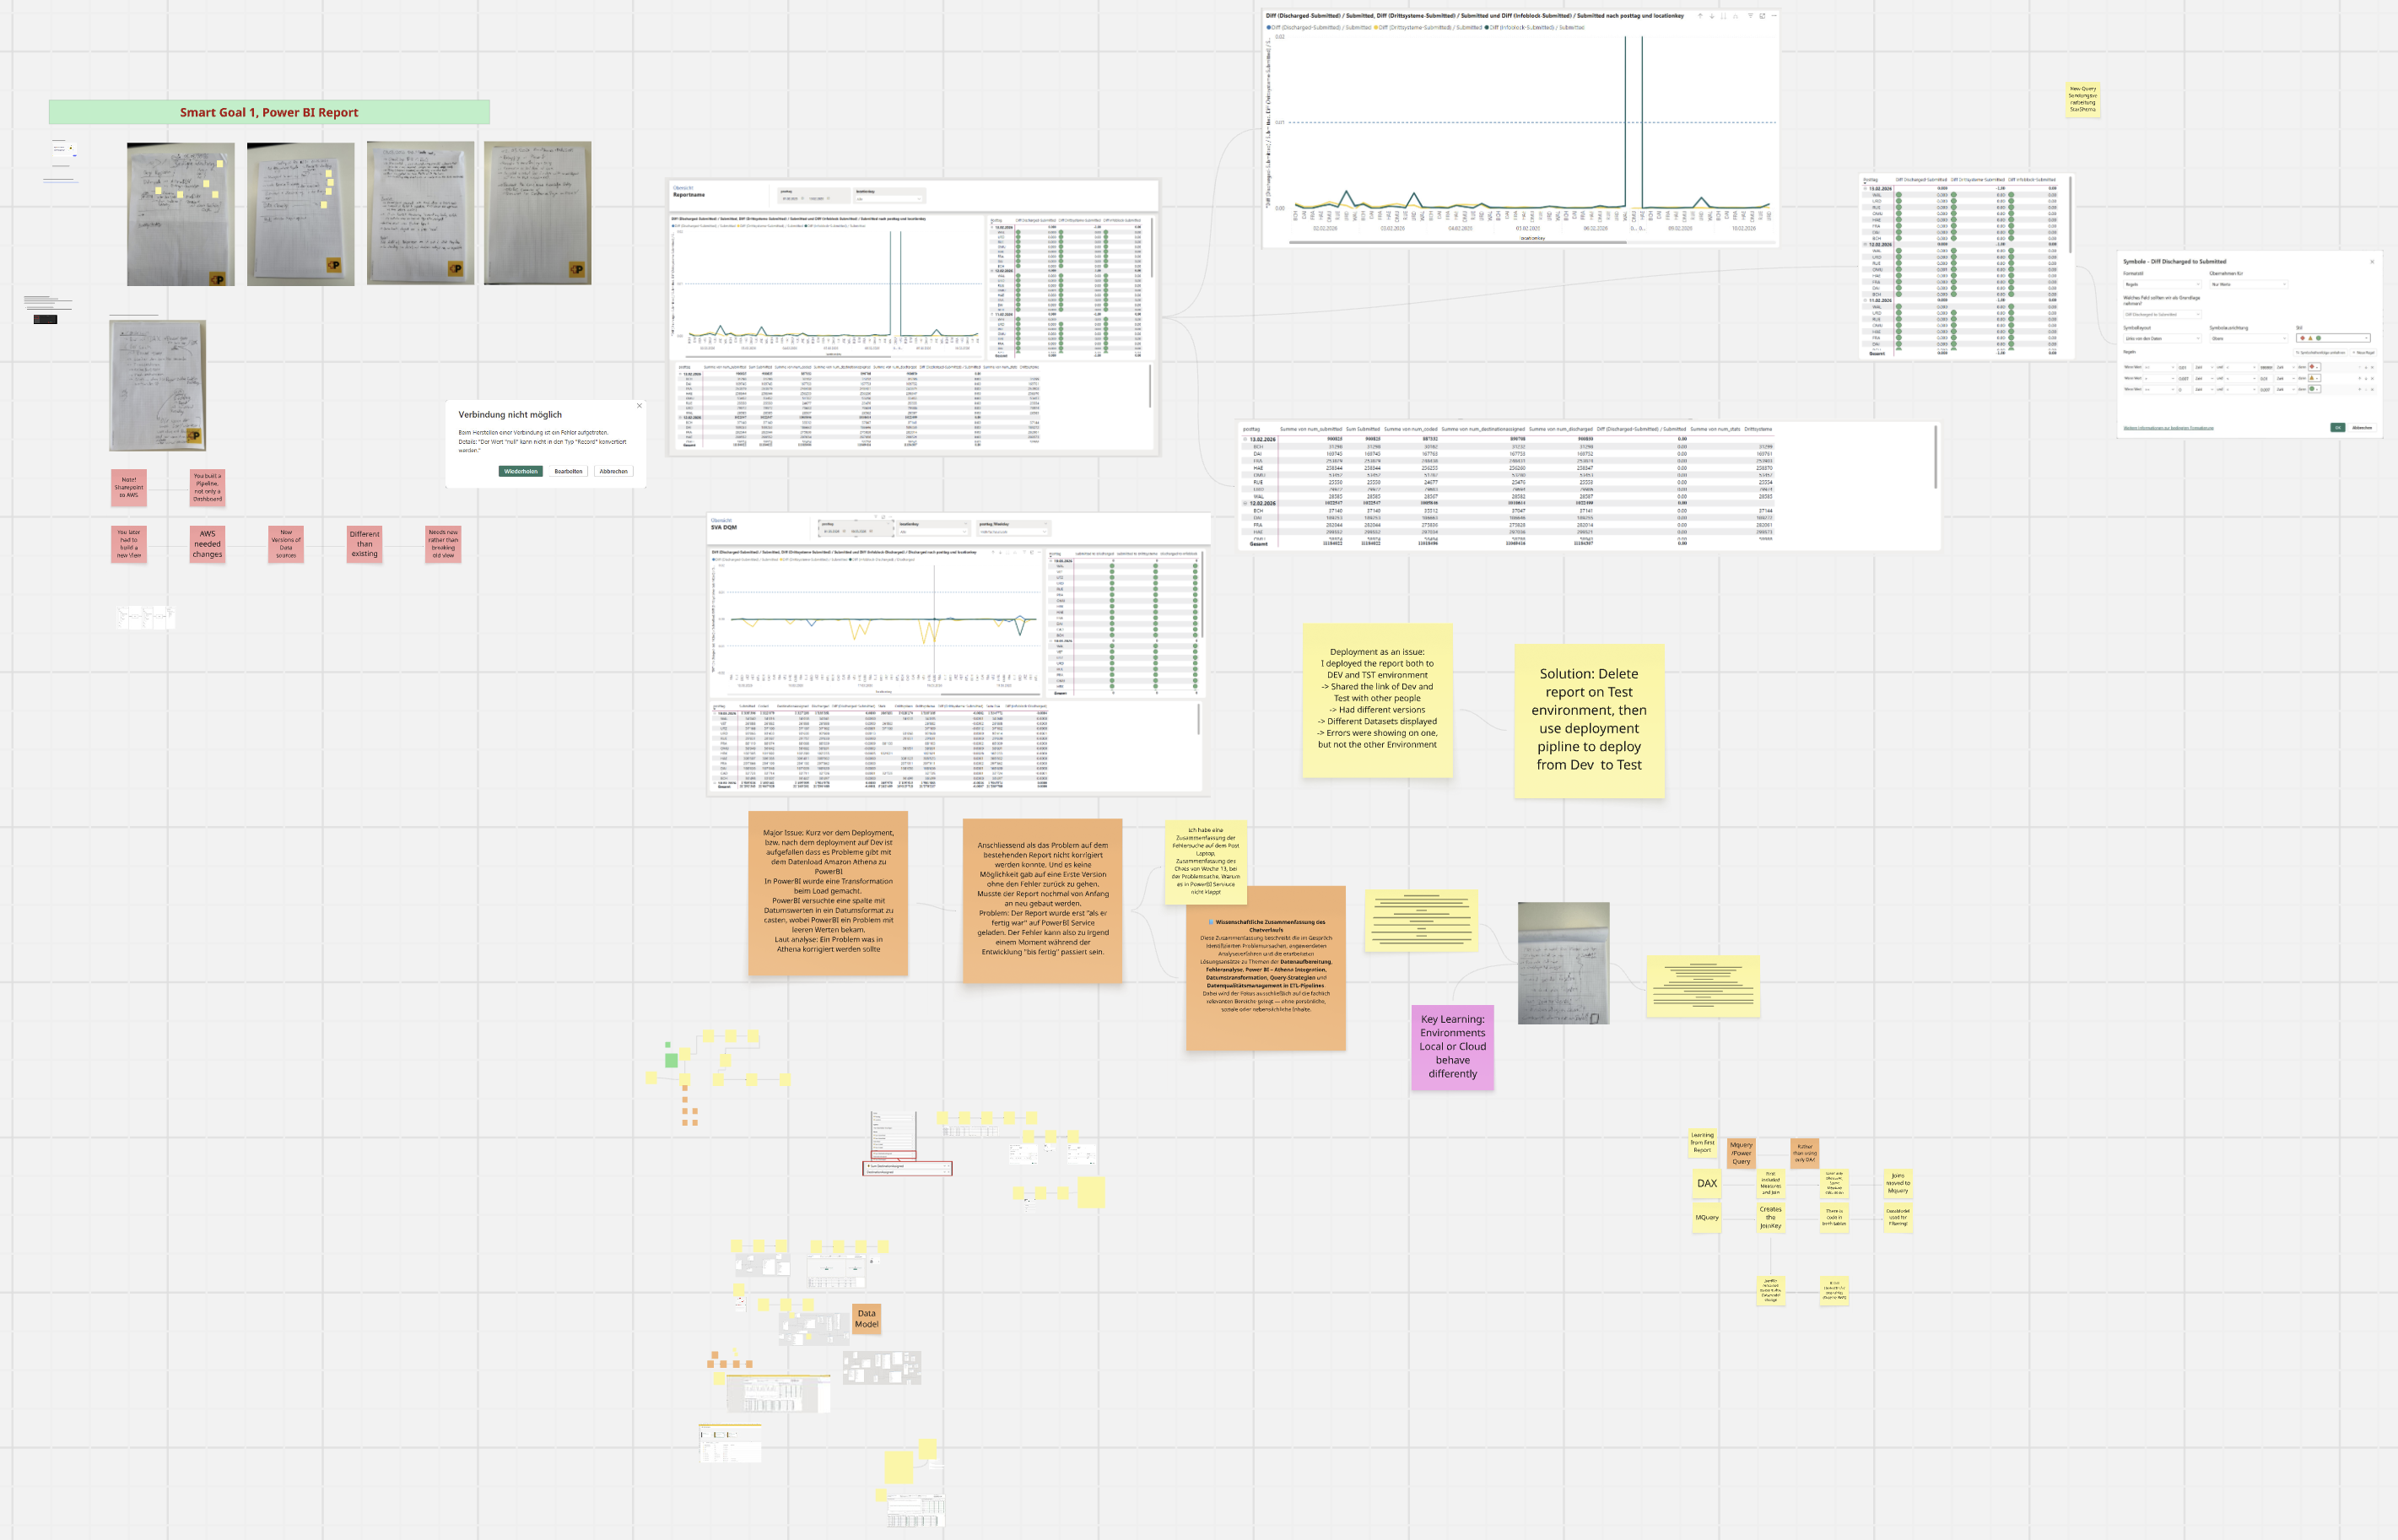
\includegraphics[width=\textwidth]{./content/img/MiroBoard_SmartGoal1.png}
    \caption{Extract of the Miro board related to Smart Goal 1. The board illustrates the planning and documentation of the reporting solution, including design concepts, implementation notes and supporting artefacts collected throughout the project.}
    \label{fig:annex_miro_smartgoal1}
\end{figure}

\begin{figure}[H]
    \centering
    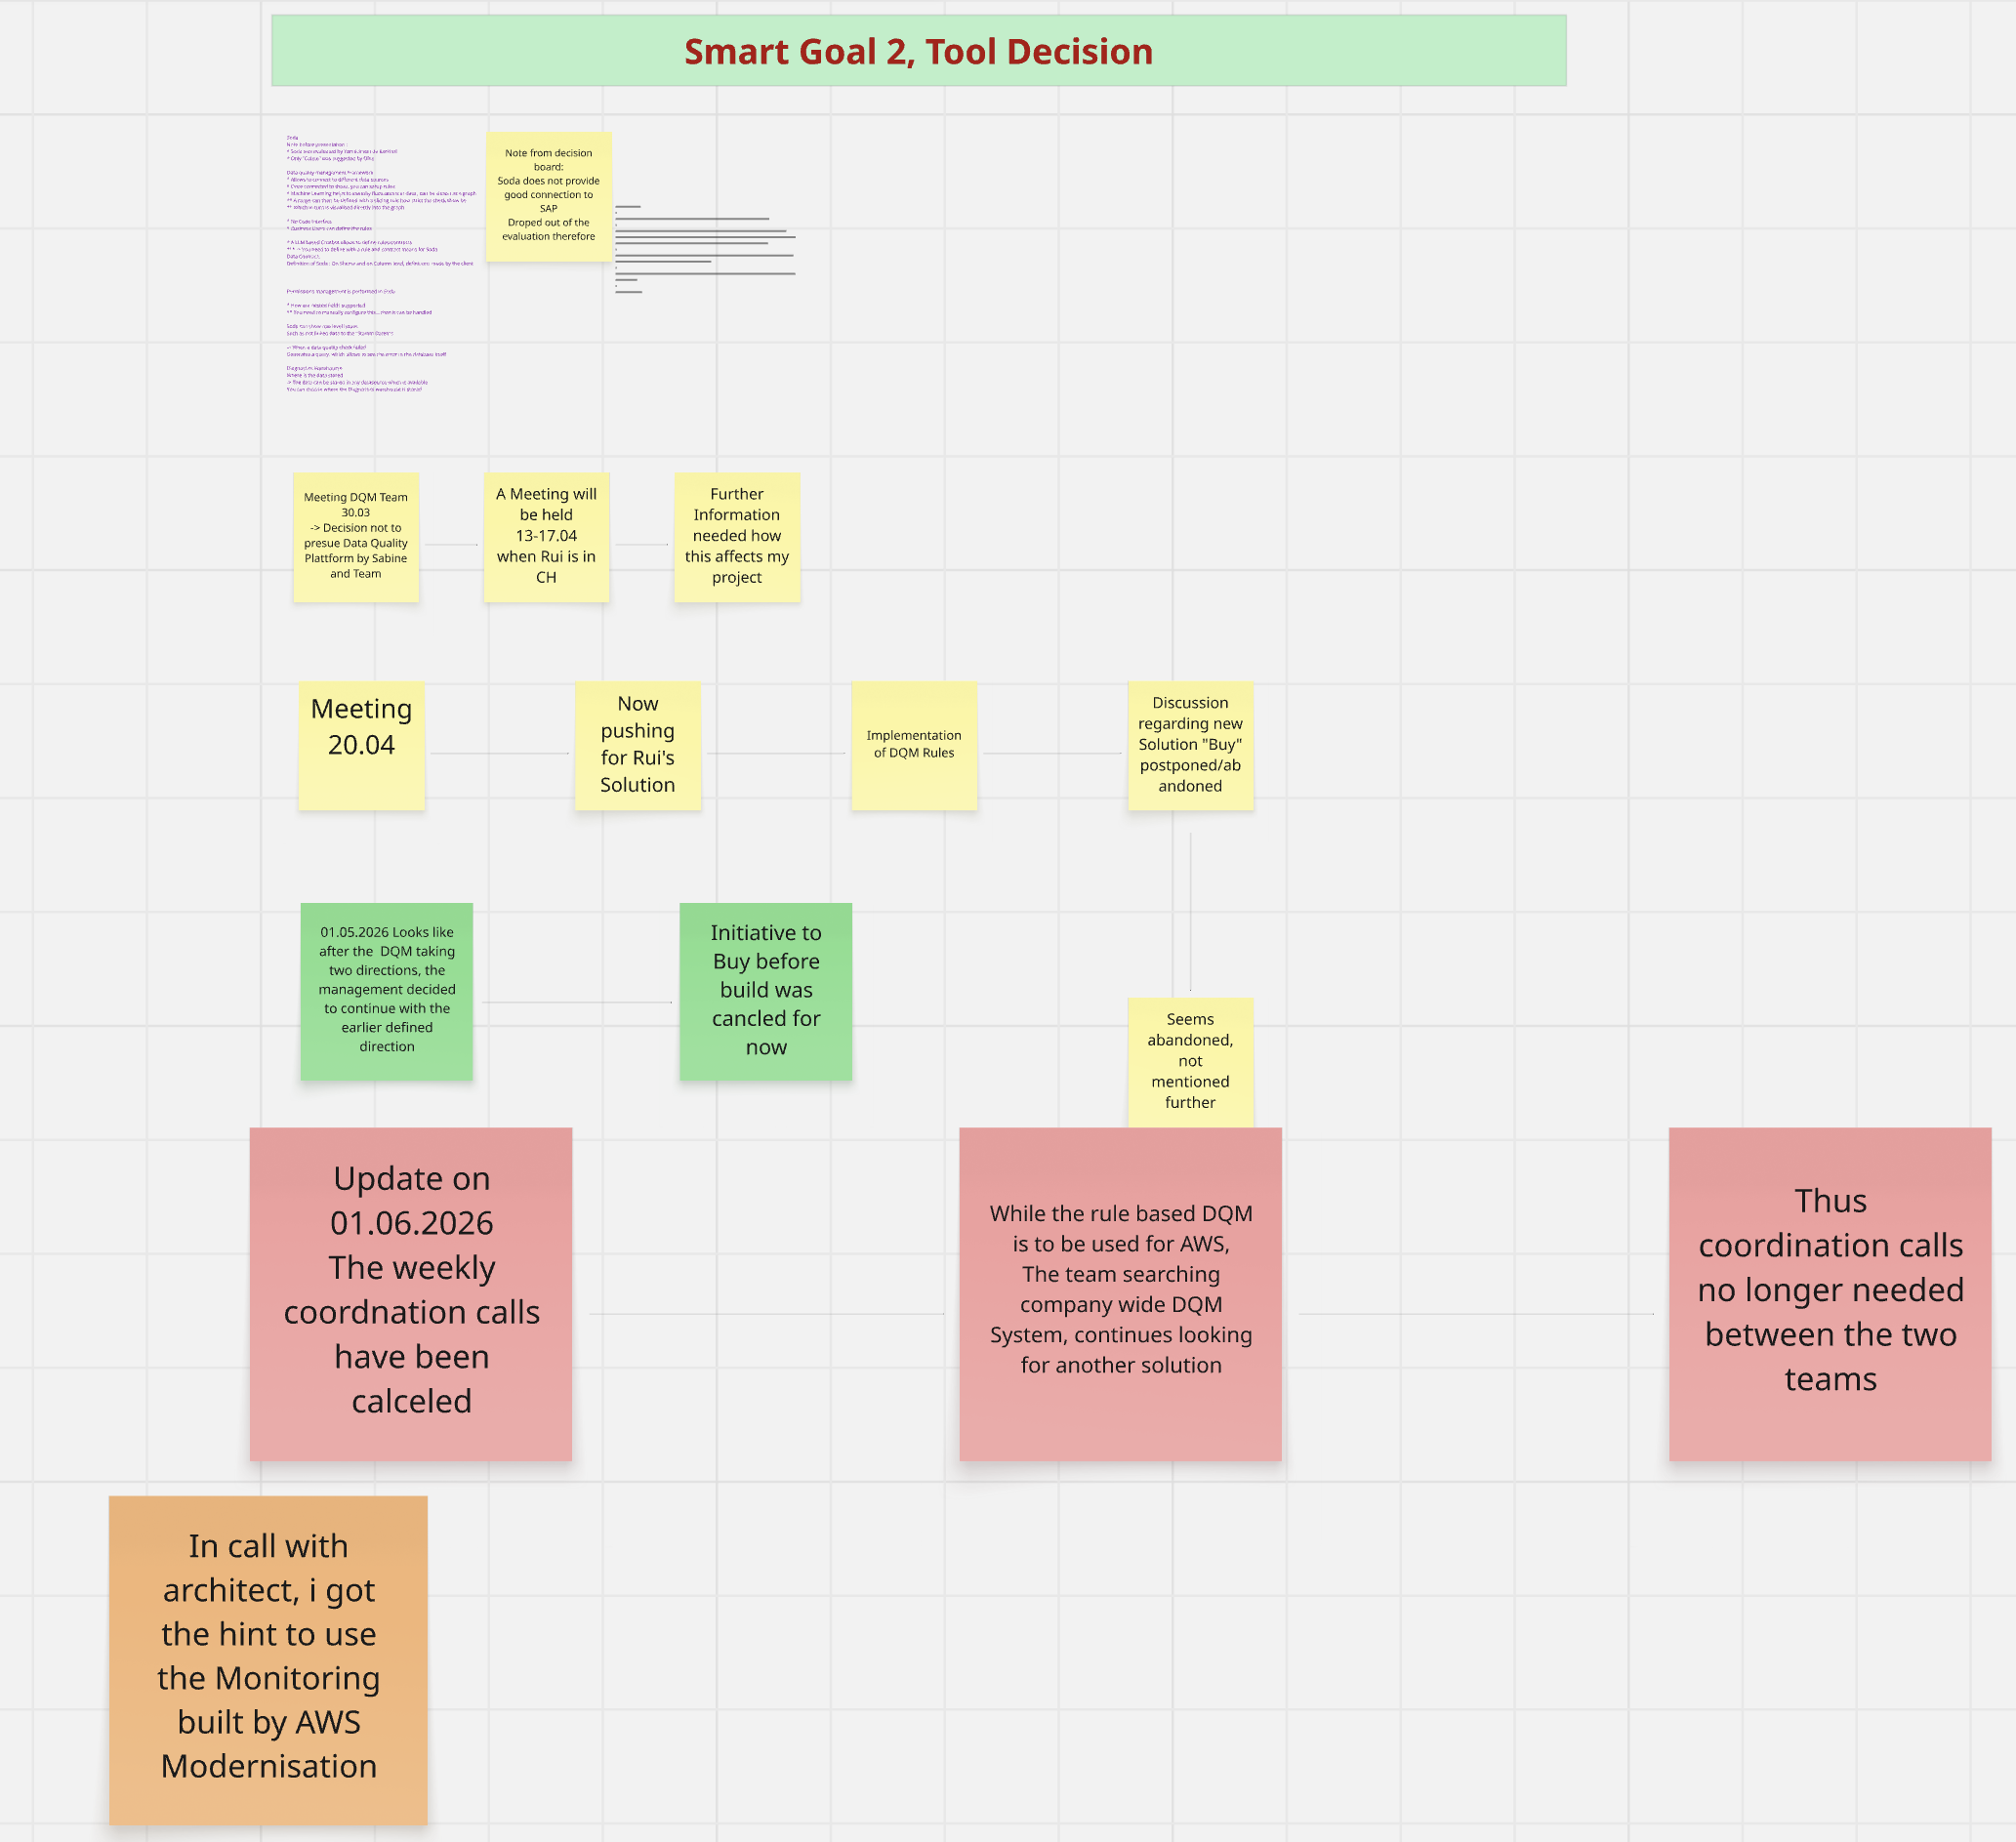
\includegraphics[width=\textwidth]{./content/img/MiroBoard_SmartGoal2.png}
    \caption{Extract of the Miro board related to Smart Goal 2. The material summarises the evaluation activities, comparisons, vendor discussions and supporting documentation used during the assessment of data quality management solutions.}
    \label{fig:annex_miro_smartgoal2}
\end{figure}

\begin{figure}[H]
    \centering
    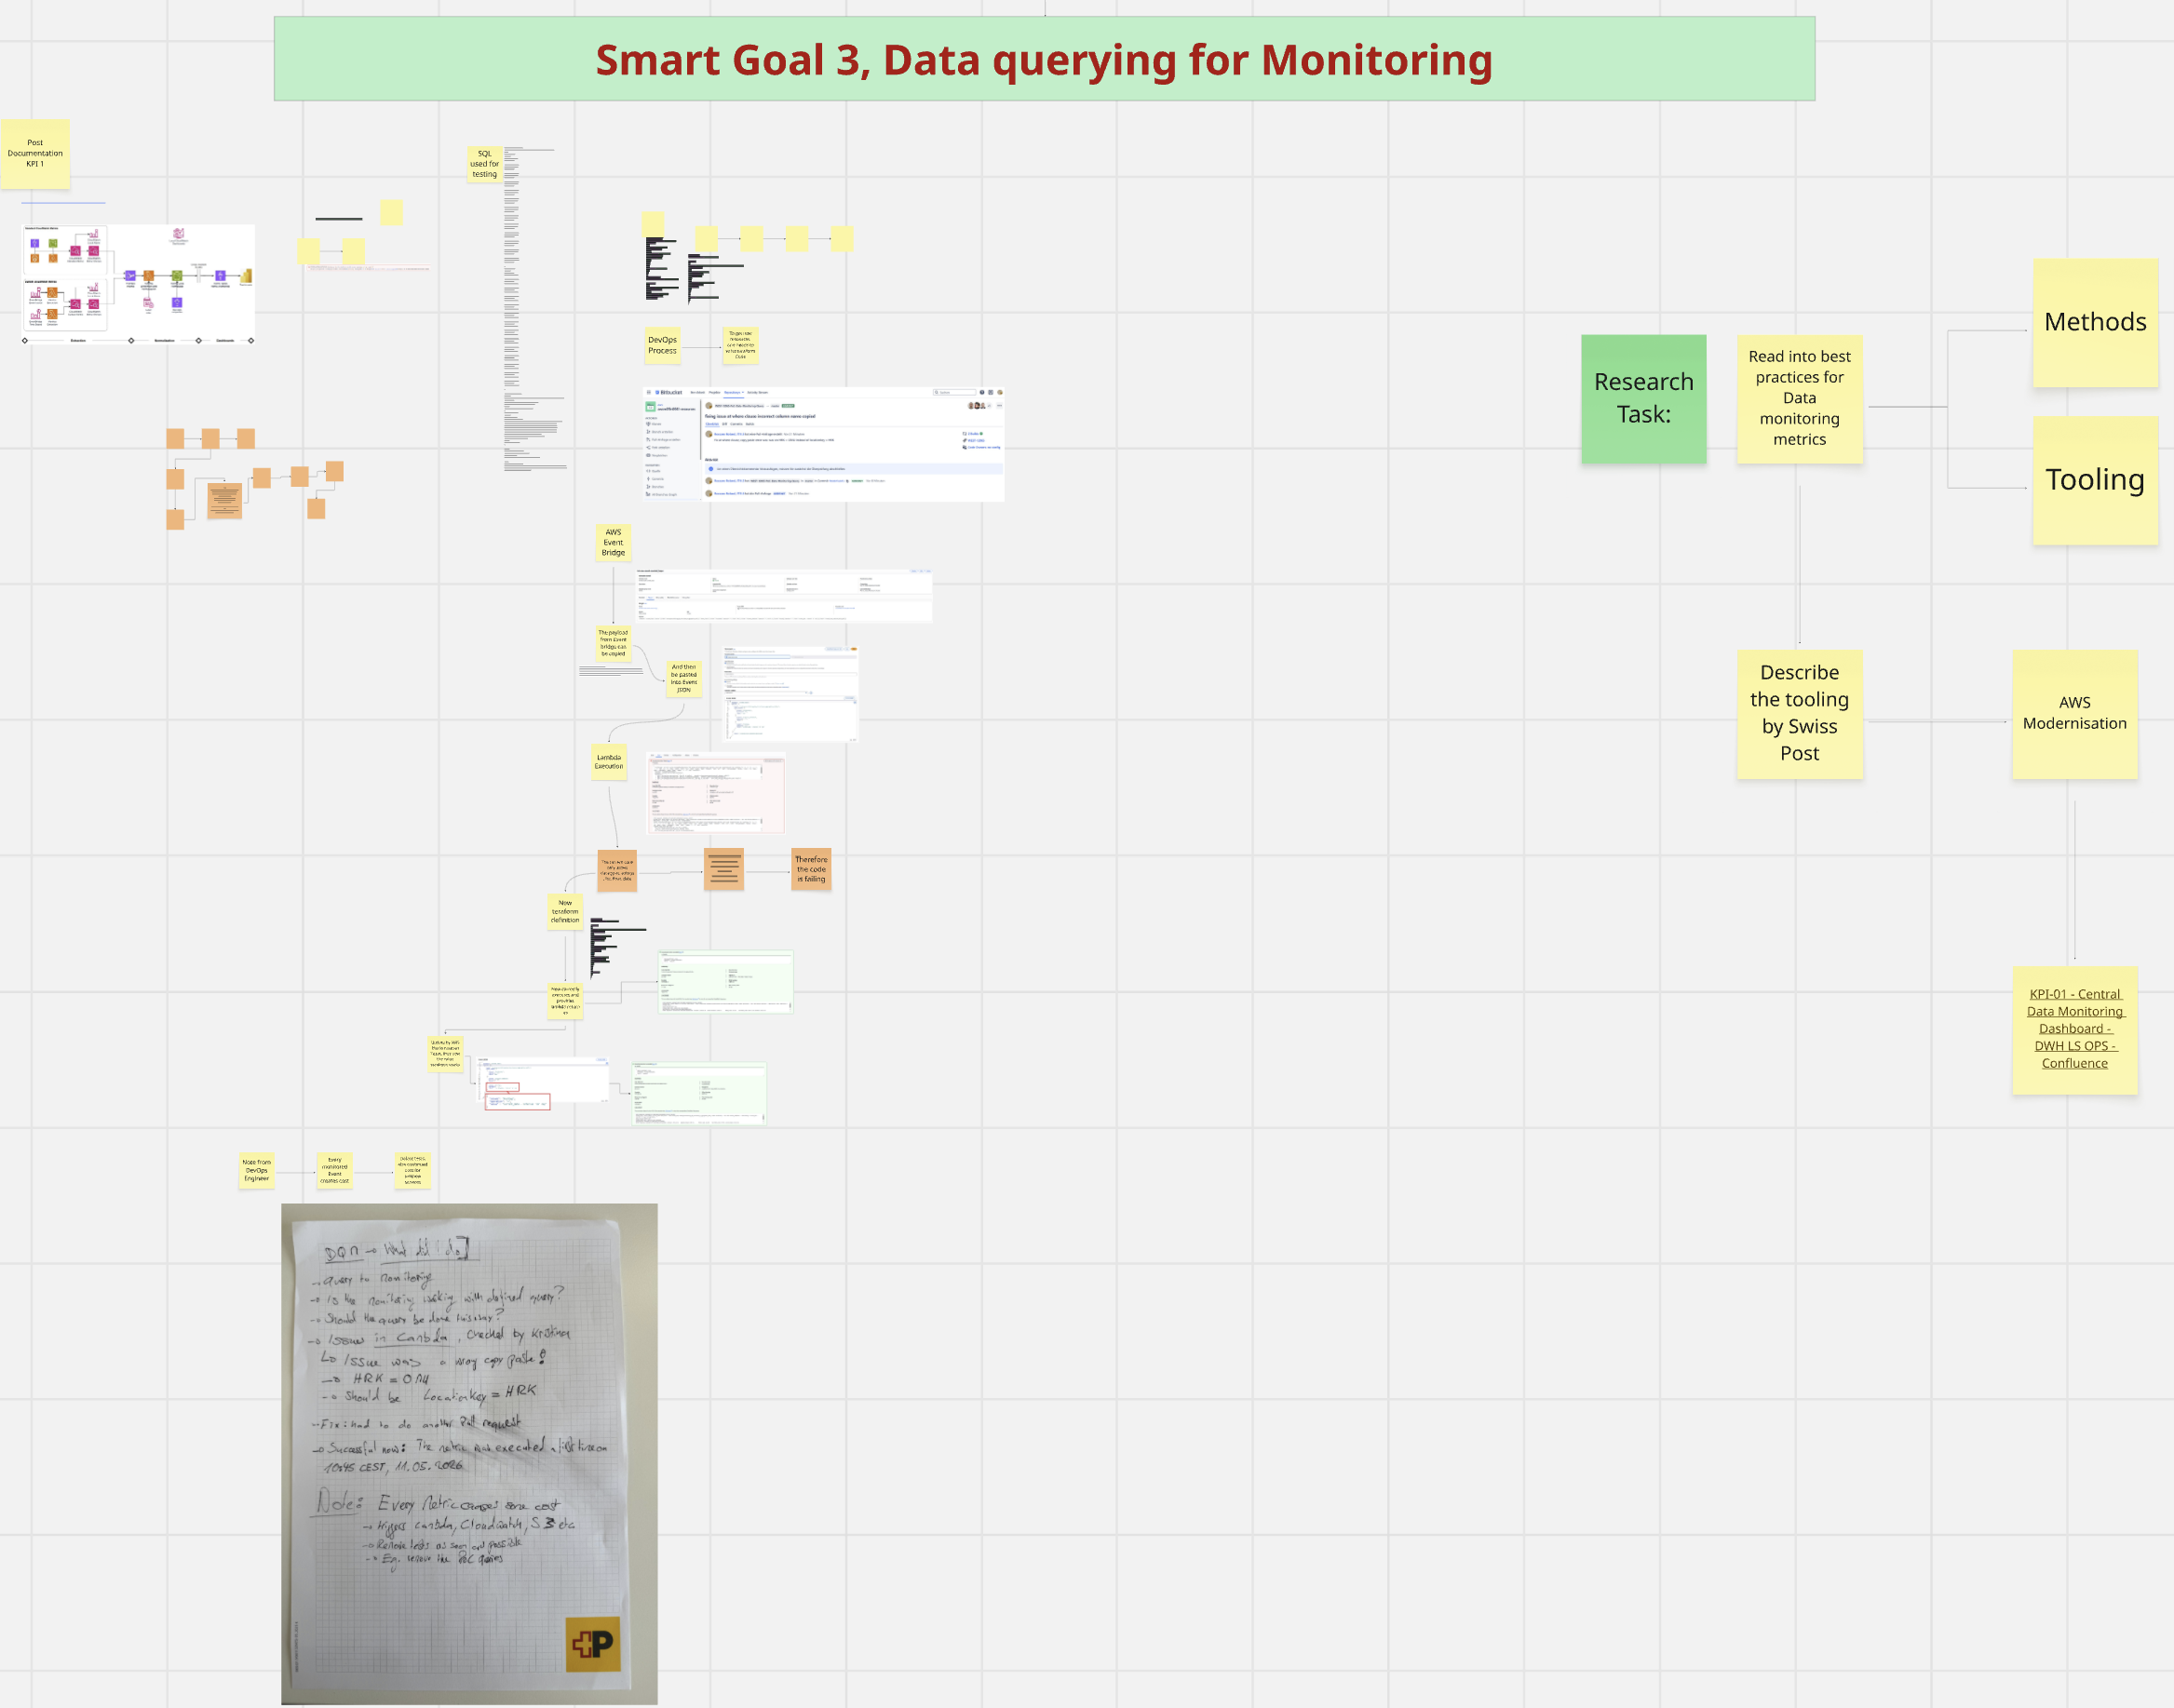
\includegraphics[width=\textwidth]{./content/img/MiroBoard_SmartGoal3.png}
    \caption{Extract of the Miro board related to Smart Goal 3. The board documents the collection of implementation notes, design ideas, intermediate results and decisions supporting the validation of the selected proof-of-concept.}
    \label{fig:annex_miro_smartgoal3}
\end{figure}